\documentclass[14pt, aspectratio=169]{beamer}
\usepackage{fontspec}
\usepackage{xcolor}
\usepackage{listings}
\usepackage{graphicx}
\usepackage{tikz}
\usepackage{adjustbox}

% fonts config
\setmainfont{DejaVu Sans}
\setsansfont{DejaVu Sans}
\setmonofont{DejaVu Sans Mono}

% colours
\definecolor{perlconf-blue}{HTML}{1E8BB3}
\setbeamercolor{itemize item}{fg=perlconf-blue}
\setbeamercolor{itemize subitem}{fg=perlconf-blue}
\setbeamercolor{itemize subsubitem}{fg=perlconf-blue}

\setbeamercolor{enumerate item}{fg=perlconf-blue}
\setbeamercolor{enumerate subitem}{fg=perlconf-blue}
\setbeamercolor{enumerate subsubitem}{fg=perlconf-blue}

\setbeamertemplate{itemize item}[triangle]
\setbeamertemplate{itemize subitem}[circle]
\setbeamertemplate{itemize subsubitem}[square]

% commands
%% insert logo from file; \logoimage[1cm]
\newcommand{\logoimage}[1][1cm]{
\includegraphics[height=#1]{include/logo.pdf}}

%% insert code from file; \inputcode{language}{filepath}
\newcommand{\inputcode}[2]{
    \begin{adjustbox}{max width=\textwidth, max height=0.8\textheight, keepaspectratio}
    \lstinputlisting[style=lststyle, showlines=true, language=#1]{#2}
    \end{adjustbox}
}

%% \position{Role, Company}
\newcommand{\position}[1]{\gdef\@position{#1}}
\newcommand{\insertposition}{\@position}

%% final frame
\newcommand{\finalframe}{
    \begin{frame}[plain]
        \centering
        \vspace{1.5cm}
        {\Large Спасибо за внимание!}
    
        \vspace{0.5cm}
        {\large Вопросы?}
        
        \vspace{0.5cm}
        \logoimage
    \end{frame}
}

%% title frame; requires \author and \title
\newcommand{\titleframe}{
    \begin{frame}[plain]
        \centering
        \vspace{1.5cm}
        {\Large\bfseries\inserttitle\par}
        \vspace{0.8cm}
        {\large\insertauthor\par}
        \vspace{0.1cm}
        {\insertposition\par}
        \vspace{0.5cm}
        \vfill
        \logoimage
    \end{frame}
}

%% author frame; requires \author and \title
\newcommand{\authorframe}[1]{
    \begin{frame}
    \begin{columns}[T,onlytextwidth]
        \begin{column}{0.39\textwidth}
            \vspace{-20mm}%
            \hspace{-10mm}%
            \begin{tikzpicture}
                \fill[color=perlconf-blue] (0,0) rectangle (\columnwidth,\paperheight+5mm);
                \begin{scope}
                    \clip (\columnwidth/2, \paperheight/2) circle (2cm);
                    \node at (\columnwidth/2, \paperheight/2) {
                        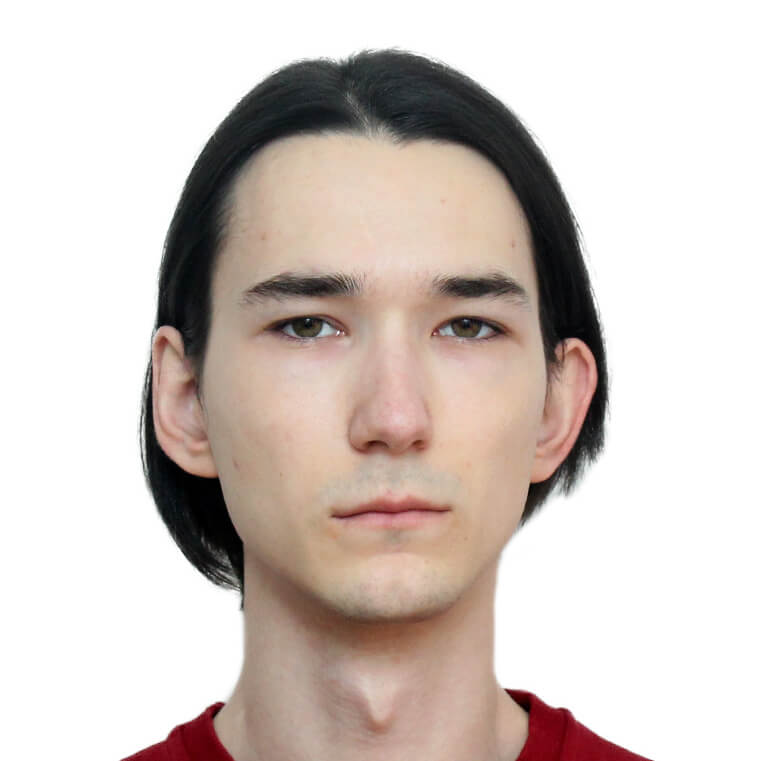
\includegraphics[width=4cm,height=4cm,keepaspectratio]{include/author.jpg}
                    };
                \end{scope}
            \end{tikzpicture}
        \end{column}
        \begin{column}{0.7\textwidth}
            \vfill
            {
                \color{perlconf-blue}
                \Large \insertauthor\par
                \vspace{0.5cm}
                \normalsize \insertposition\par
                \vspace{0.5cm}
            }
            #1
            \vfill
        \end{column}
    \end{columns}
    \end{frame}
}

% END of commands

% hide navigation
\setbeamertemplate{navigation symbols}{}

% frame page numbers config
\setbeamertemplate{footline}{%
    \hfill\large\color{perlconf-blue}\insertframenumber%
    \hspace{0.5cm}\vspace{0.5cm}%
}

% frame logo config
\setbeamertemplate{headline}{%
    \vspace{0.5cm}
    \hfill
    \logoimage[0.7cm]
    \hspace{0.3cm}
	\hfill
}

% frame header config
\setbeamertemplate{frametitle}{%
    \vspace{-0.8cm}%
    \hspace{-0.5cm}%
    \large\color{perlconf-blue}\insertframetitle%
}

% lstlistings config
\lstdefinestyle{lststyle}{
    basicstyle=\ttfamily\footnotesize,
    breaklines=true,
    numbers=left,
    numberstyle=\tiny\color{gray},
    keywordstyle=\color{perlconf-blue}\bfseries,
    commentstyle=\color{green!50!black},
    stringstyle=\color{red!50!black},
    showstringspaces=false,
    tabsize=4,
    frame=none,
    xleftmargin=10pt,
    xrightmargin=10pt
}

\lstdefinelanguage{XS}{
    morekeywords={MODULE, PACKAGE, PREFIX, CODE, OUTPUT, INIT, PREINIT, CLEANUP},
    sensitive=true,
    morecomment=[l]{\#},
    morestring=[b]{"}
}

\lstdefinelanguage{XStypemap}{
    morekeywords={TYPEMAP, INPUT, OUTPUT},
    sensitive=true,
    morecomment=[l]{\#},
    morestring=[b]{"}
}

\title{Описание typemap для передачи структур в XS}
\author{Ступницкий Иван}
\position{Инженер, YADRO}
\begin{document}
\titleframe

% Plan
\begin{frame}[fragile]{О чём расскажу}
    \begin{enumerate}
        \item Кто я
        \item Problem?
        \item XS в двух словах
        \item Как переводится название доклада
        \item Подопытная библиотека
        \item В чём вообще проблема
        \item Способы передачи структур в XS
        \item Передача структур из XS в Perl
        \item Как и что в итоге использовать
    \end{enumerate}
\end{frame}

% Author frame
\authorframe{
    \begin{itemize}
        \item Два года программирую\\ на Perl за деньги\\~
        \item Увлекаюсь информационной безопасностью и сложными системами
    \end{itemize}
}

\begin{frame}[fragile]{Мотивация к докладу}
    \centering
    
\includegraphics[width=.4\textwidth]{snippets/xorg_logo.png}\hfill
    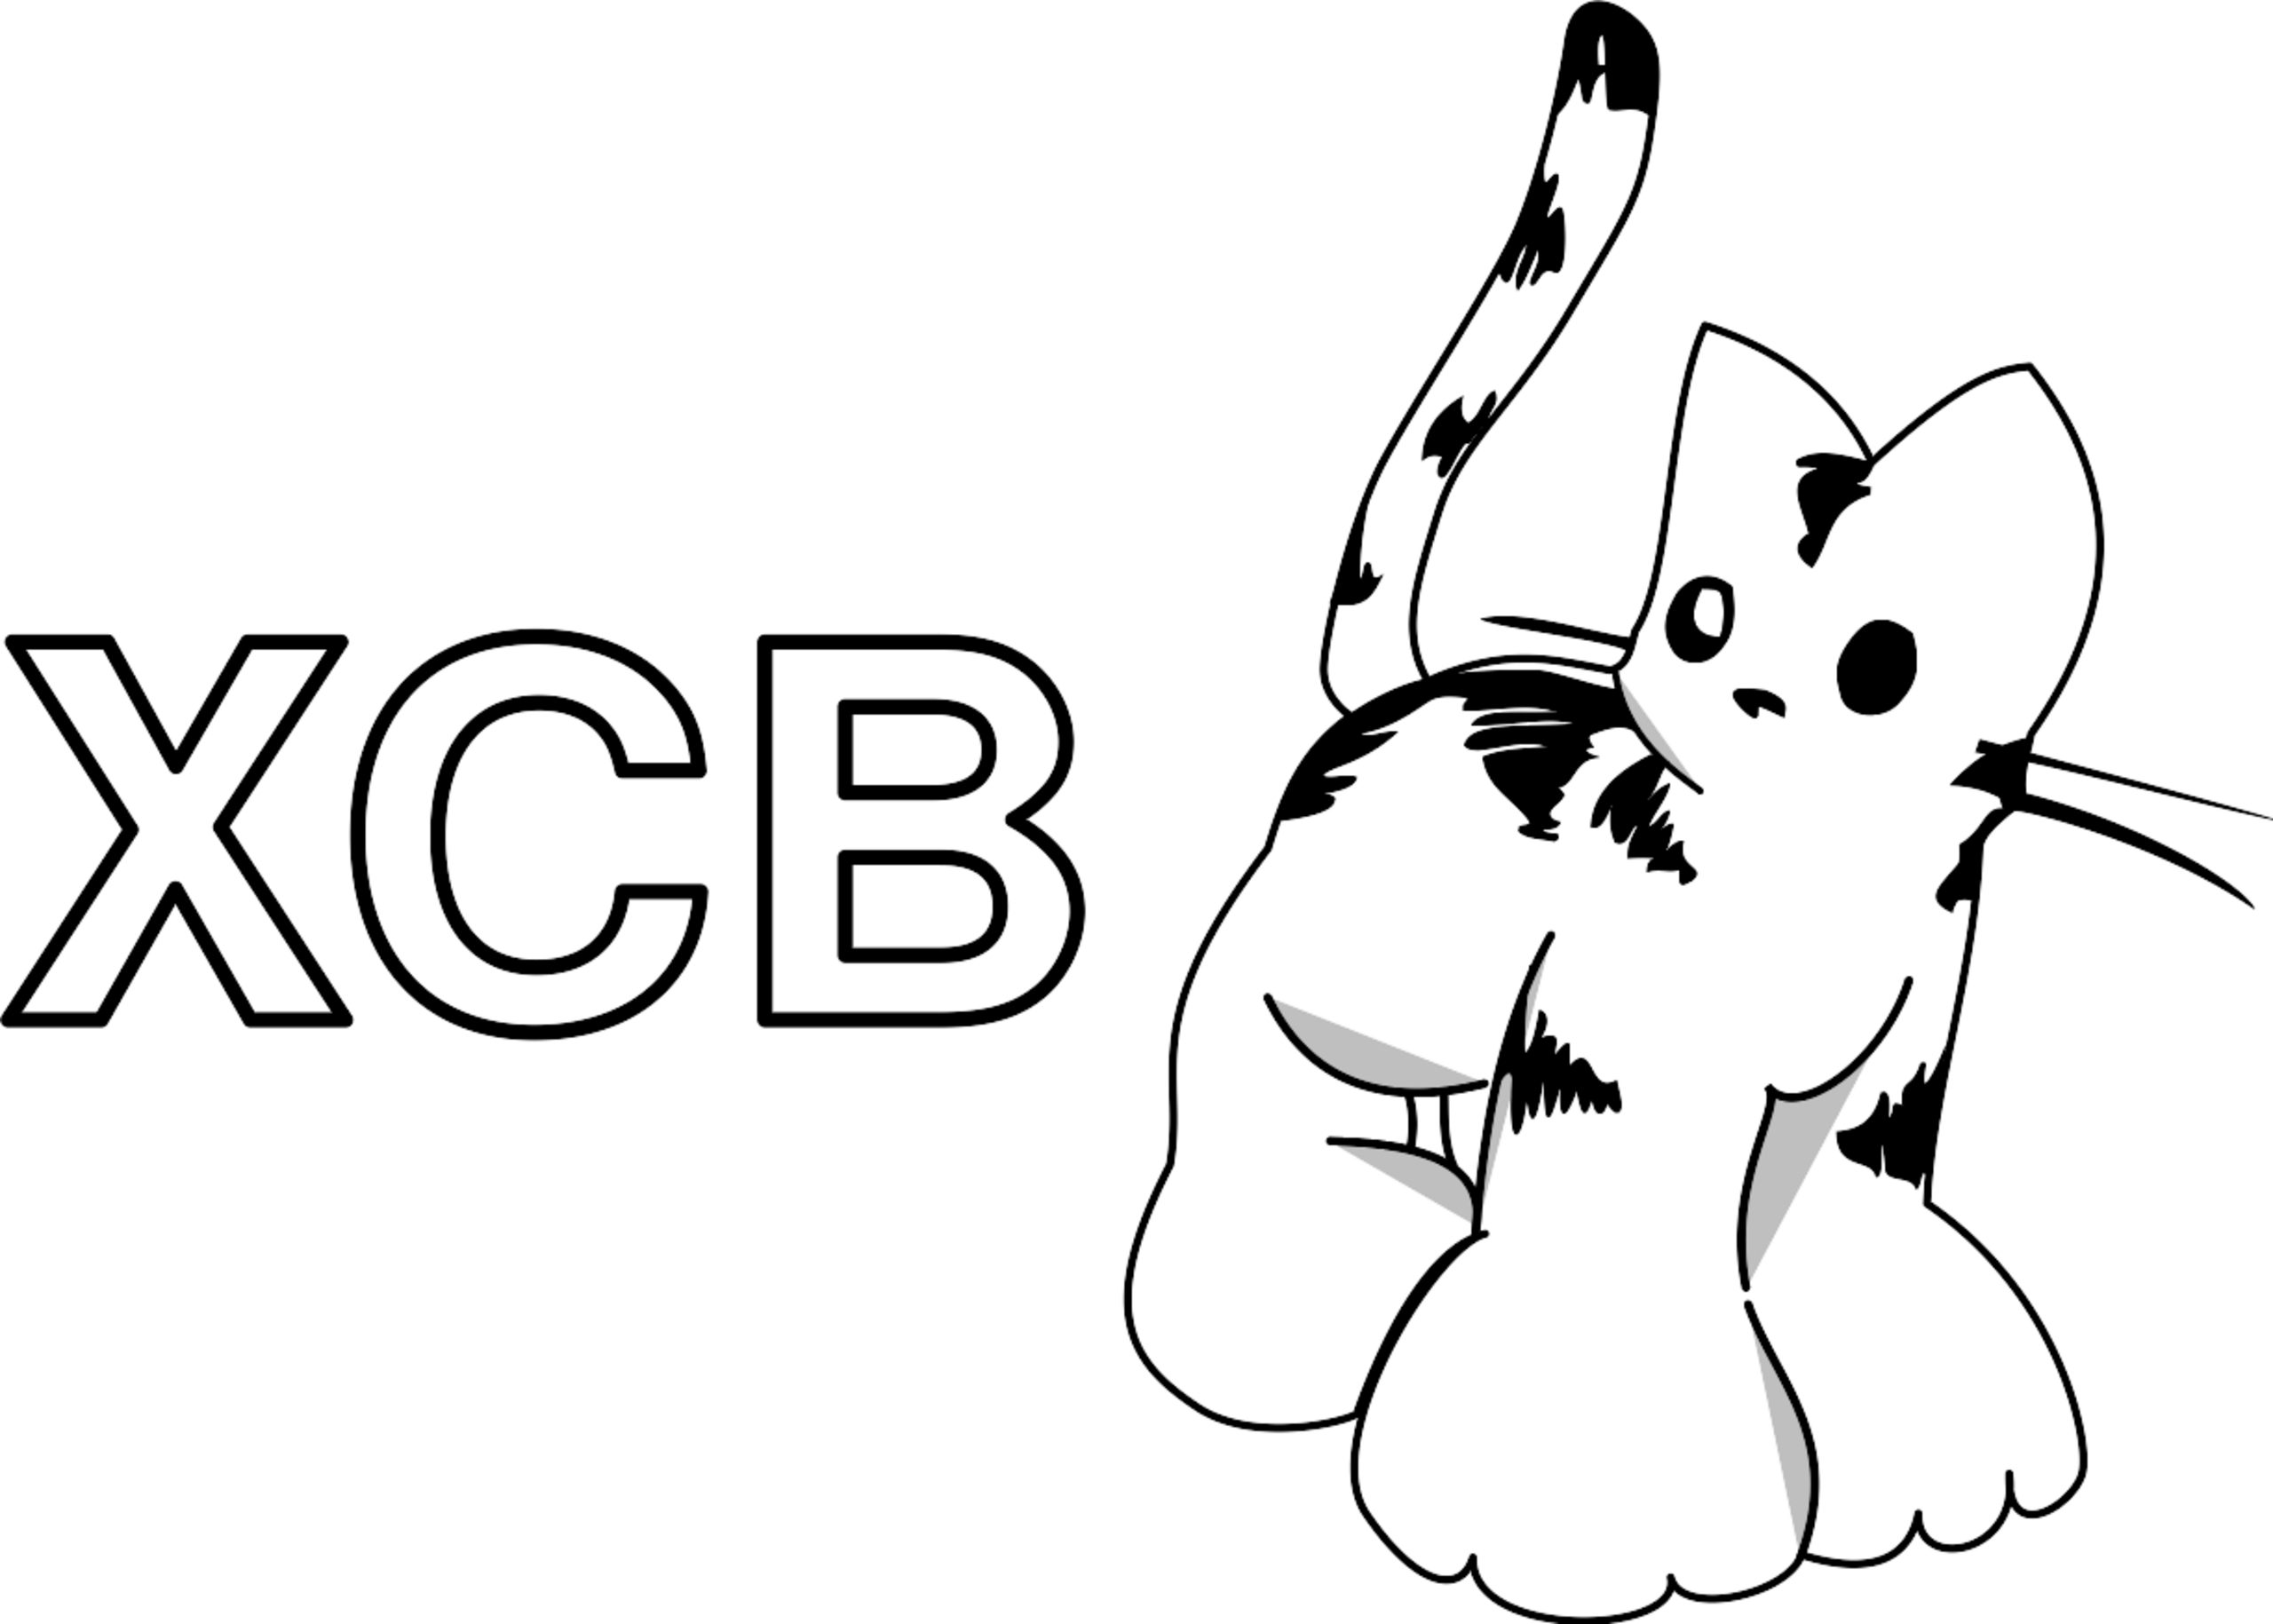
\includegraphics[width=.4\textwidth]{snippets/xcb_logo.png}\hfill
\end{frame}

\begin{frame}[fragile]{Мотивация к докладу}
    \inputcode{C}{snippets/xcb_randr_mode_info_t.c}
\end{frame}

\begin{frame}[fragile]{Мотивация к докладу}
    \inputcode{C}{snippets/xcb_randr_create_mode.c}
\end{frame}

\begin{frame}[fragile]{Мотивация к докладу}
    \inputcode{Perl}{snippets/korgwm_xs_example.pl}
\end{frame}

\begin{frame}[fragile]{Что почитать про XS}
    \begin{itemize}
        \setlength\itemsep{1em}
        \item \texttt{perlxstut}
        \item \texttt{perlxs}
        \item \texttt{perlguts}
        \item \texttt{perlapi}
        \item \texttt{perlxstypemap}
    \end{itemize}
\end{frame}

\begin{frame}[fragile]{XS в двух словах}
    \only<1>{
        \inputcode{txt}{snippets/xs-quick-start.txt}
    }
    \only<2>{
        \inputcode{txt}{snippets/xs-quick-start-comments.txt}
    }
\end{frame}

\begin{frame}[fragile]{Основной модуль}
    \inputcode{Perl}{snippets/xs-basic-lib.pl}
\end{frame}

\begin{frame}[fragile]{Mytest.xs}
    \inputcode{XS}{snippets/Mytest.xs}
\end{frame}

\begin{frame}[fragile]{Makefile.PL}
    \inputcode{Perl}{snippets/Makefile.PL}
\end{frame}

\begin{frame}[fragile]{Как переводится название доклада}
    \centering
    \hspace{0.5cm}
    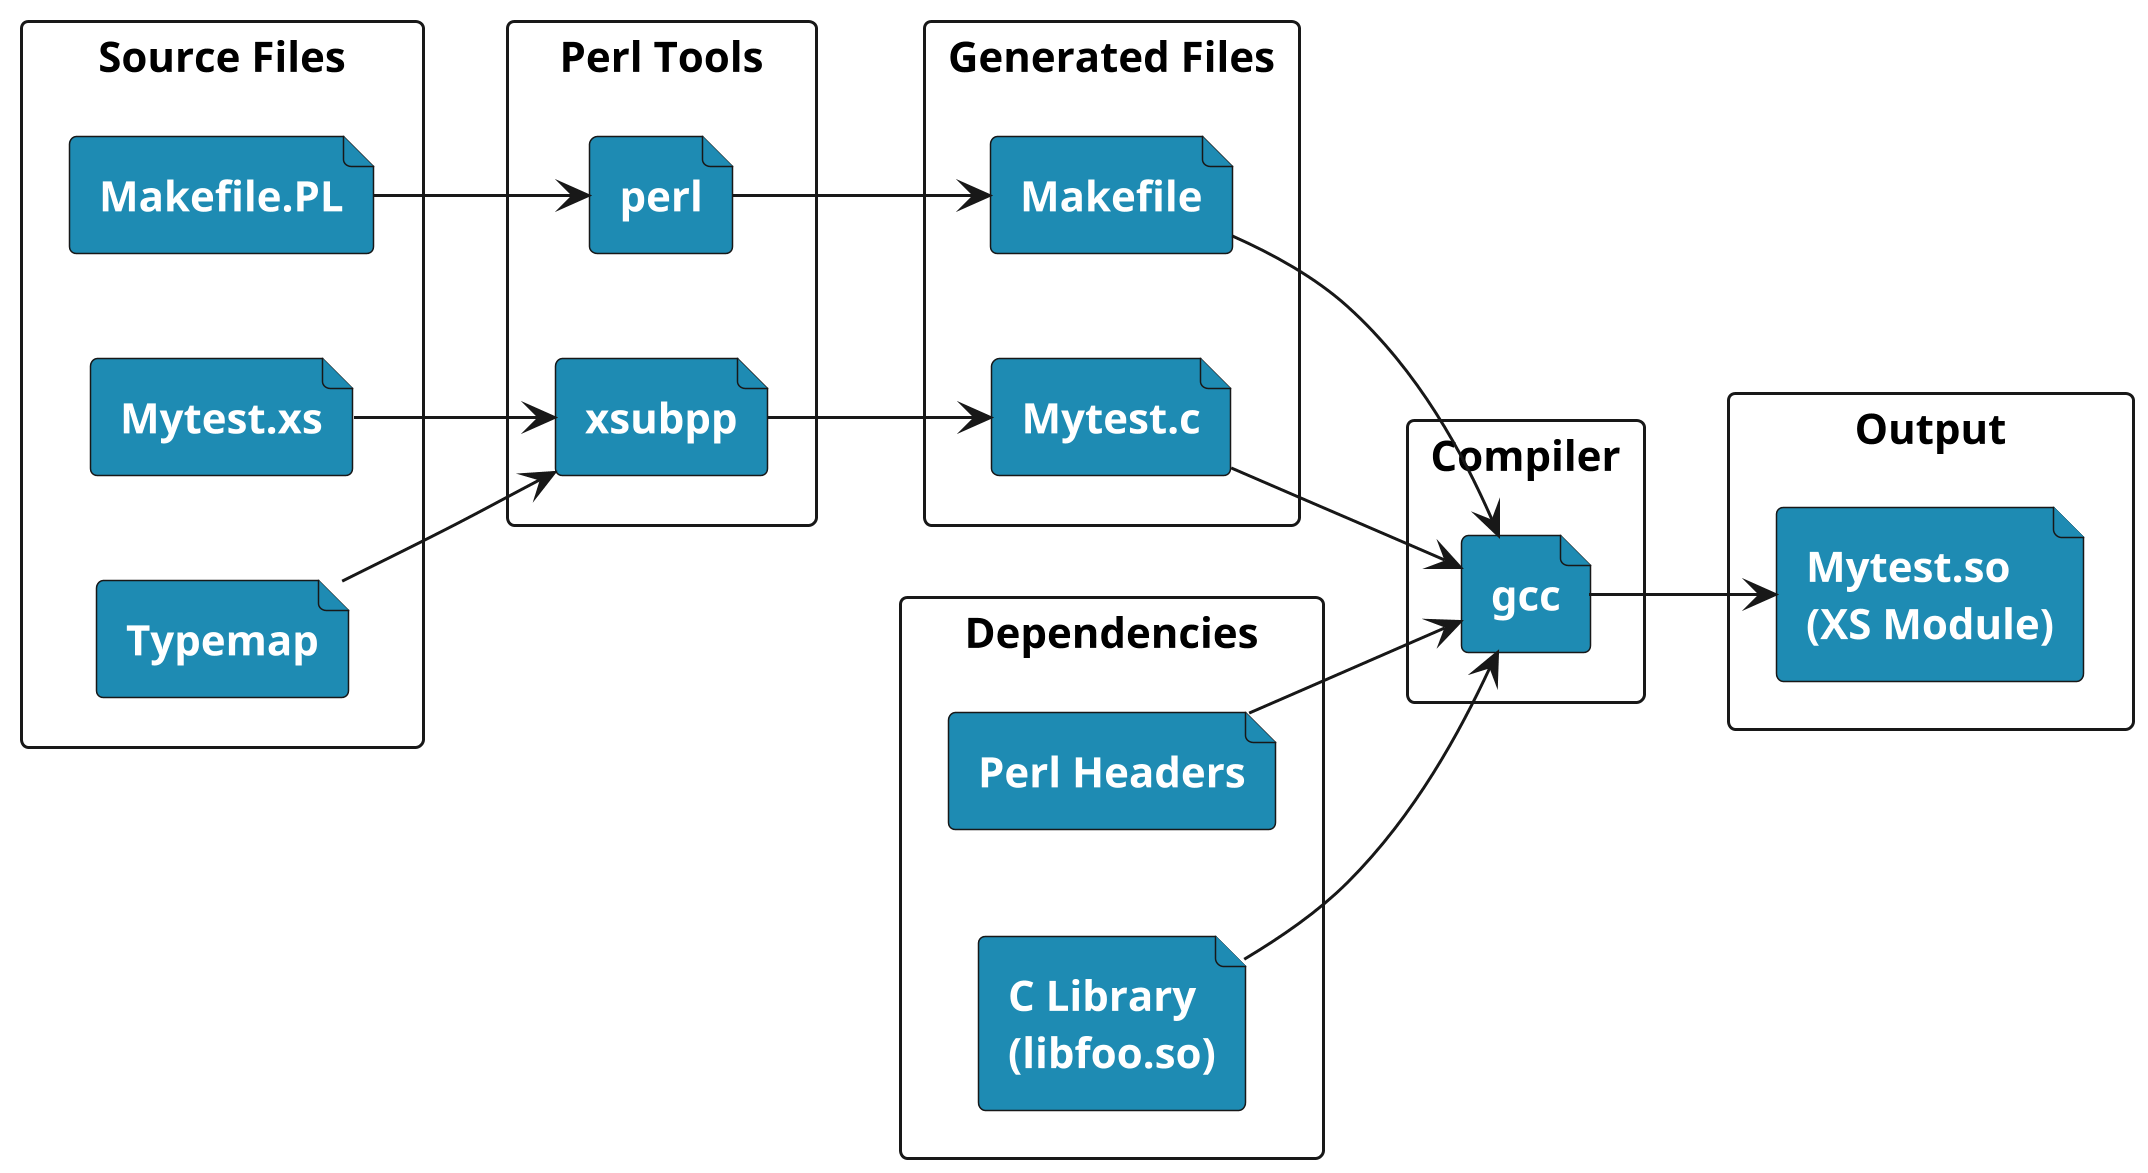
\includegraphics[height=\textheight]{snippets/xs-compilation-scheme.png}
\end{frame}

\begin{frame}[fragile]{Подопытная библиотека libfoo}
    \inputcode{C}{snippets/foo-simple.c}
    \par\vspace{0.5cm}
    \inputcode{C}{snippets/foo-simple.h}
\end{frame}

\begin{frame}[fragile]{Вызов libfoo из Си}
    \inputcode{C}{snippets/bar-simple.c}
    \par\vspace{0.5cm}
    \inputcode{txt}{snippets/bar-output.txt}
\end{frame}

\begin{frame}[fragile]{Вызов libfoo из XS}
    \inputcode{XS}{snippets/xs-1.xs}
\end{frame}

\begin{frame}[fragile]{Makefile.PL}
    \only<1>{
        \inputcode{Perl}{snippets/Makefile.PL}
    }
    \only<2>{
        \inputcode{Perl}{snippets/Makefile-1.PL}
    }
\end{frame}

\begin{frame}[fragile]{Тестирование}
    \inputcode{Perl}{snippets/test-1.pl}

    \onslide<2->{
        \vspace{0.5cm}
        \inputcode{txt}{snippets/out-1.txt}
    }
\end{frame}

\begin{frame}[fragile]{Структура в libfoo}
    \inputcode{C}{snippets/foo-struct.c}

    \onslide<2->{
        \vspace{0.5cm}
        \inputcode{C}{snippets/foo-struct.h}
    }
\end{frame}

\begin{frame}[fragile]{Вот и всё!\onslide<4->{ (нет)}}
    \inputcode{XS}{snippets/xs-2.xs}

    \onslide<2->{
        \vspace{0.5cm}
        \inputcode{Perl}{snippets/test-2.pl}
    }

    \onslide<3->{
        \vspace{0.5cm}
        \inputcode{txt}{snippets/out-2.txt}
    }
\end{frame}

\begin{frame}[fragile]{В XS нужно проще}
    \inputcode{XS}{snippets/xs-1a.xs}

    \onslide<2->{
        \vspace{0.5cm}
        \inputcode{Perl}{snippets/test-1a.pl}
    }

    \onslide<3->{
        \vspace{0.5cm}
        \inputcode{txt}{snippets/out-1.txt}
    }
\end{frame}

\begin{frame}[fragile]{А теперь со структурой}
    \inputcode{XS}{snippets/xs-3.xs}

    \onslide<2->{
        \vspace{0.25cm}
        \inputcode{txt}{snippets/out-3.txt}
    }
\end{frame}

\begin{frame}[fragile]{Что такое typemap}
    \centering
    \hspace{0.5cm}
    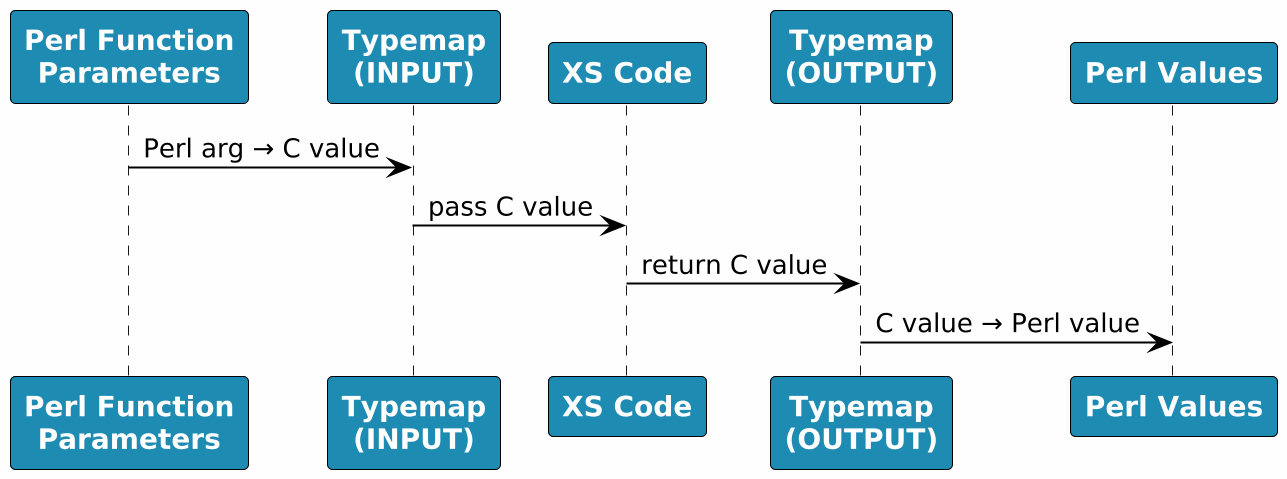
\includegraphics[width=\textwidth]{snippets/typemap-scheme.png}
\end{frame}

\begin{frame}[fragile]{Что такое typemap}
    \onslide<1->{}
    \onslide<4->{
        \inputcode{XStypemap}{snippets/typemap-basic-typemap}
    }

    \onslide<2->{
        \vspace{0.25cm}
        \inputcode{XStypemap}{snippets/typemap-basic-input}
    }

    \onslide<3->{
        \vspace{0.25cm}
        \inputcode{XStypemap}{snippets/typemap-basic-output}
    }
\end{frame}

\begin{frame}[fragile]{T\_PACKED}
    \inputcode{XStypemap}{snippets/typemap-4}

    \onslide<2->{
        \vspace{0.5cm}
        \inputcode{XS}{snippets/xs-4.xs}
    }
\end{frame}

\begin{frame}[fragile]{T\_PACKED fuckup}
    \inputcode{txt}{snippets/out-4.txt}
\end{frame}

\begin{frame}[fragile]{Фикс для T\_PACKED}
    \inputcode{XStypemap}{snippets/typemap-4a}

    \onslide<2->{
        \vspace{0.5cm}
        \inputcode{txt}{snippets/out-4a.txt}
    }
\end{frame}

\begin{frame}[fragile]{Как это выглядит в Си}
    \inputcode{C}{snippets/xs-4.c}
\end{frame}

\begin{frame}[fragile]{Избежать вызова функции}
    \inputcode{XStypemap}{snippets/typemap-5}

    \onslide<2->{
        \vspace{0.5cm}
        \inputcode{txt}{snippets/out-5.txt}
    }
\end{frame}

\begin{frame}[fragile]{Как это выглядит в Си}
    \inputcode{C}{snippets/xs-5.c}
\end{frame}

\begin{frame}[fragile]{Передача структуры C -> Perl [1]}
    \inputcode{C}{snippets/xs-5-fooGet.c}

    \onslide<2->{
        \vspace{0.5cm}
        \inputcode{C}{snippets/xs-5-fooGet.h}
    }

    \onslide<3->{
        \vspace{0.5cm}
        \inputcode{XS}{snippets/xs-5-fooGet.xs}
    }
\end{frame}

\begin{frame}[fragile]{Передача структуры C -> Perl [2]}
    \inputcode{XStypemap}{snippets/xs-5-fooGet-typemap}
\end{frame}


\begin{frame}[fragile]{Передача структуры C -> Perl [3]}
    \inputcode{Perl}{snippets/xs-5-fooGet-test.pl}

    \onslide<2->{
        \vspace{0.5cm}
        \inputcode{txt}{snippets/xs-5-fooGet-out.txt}
    }
\end{frame}

\begin{frame}[fragile]{Как это выглядит в Си}
    \inputcode{C}{snippets/xs-5-fooGet-xsc.c}
\end{frame}

\begin{frame}[fragile]{А теперь без хардкода}
    \inputcode{XStypemap}{snippets/typemap-6}

    \onslide<2->{
        \vspace{0.5cm}
        \inputcode{Perl}{snippets/test-6.pl}
    }

    \onslide<3->{
        \vspace{0.5cm}
        \inputcode{txt}{snippets/out-6.txt}
    }
\end{frame}

\begin{frame}[fragile]{Финальный typemap [1]}
    \inputcode{XStypemap}{snippets/typemap-final-1}
\end{frame}

\begin{frame}[fragile]{Финальный typemap [2]}
    \inputcode{XStypemap}{snippets/typemap-final-2}
\end{frame}

\begin{frame}[fragile]{Финальный typemap [3]}
    \inputcode{Perl}{snippets/test-final.pl}

    \onslide<2->{
        \vspace{0.5cm}
        \inputcode{txt}{snippets/out-final.txt}
    }
\end{frame}

\begin{frame}[fragile]{Выводы}
    В простом случае можно описывать код в функциях на Си и использовать T\_PACKED\textcolor{gray}{\_PATCHED}
    => компилятор сделает работу за вас :)
    \vspace{0.5cm}

    При работе со сложными структурами или для\\
    явного контроля трансляции предпочтительнее написать typemap
\end{frame}

\finalframe
\end{document}
